\documentclass[xcolor=table, 11pt, aspectratio=169]{beamer}

%\usepackage{arev}
\usepackage{amsmath,amssymb,amscd}
\usepackage{dsfont}
\usepackage{mathrsfs}
\usepackage{yfonts}
\usepackage{bm}
\usepackage{graphicx}
\usepackage{tabularx}
\usepackage{animate}
\usepackage{listings}
\usepackage{pifont}
%\usepackage{mathtools}
%\usepackage{ifthen}

%\usepackage{xeCJK}
%\usepackage{fontspec}
%\newfontfamily\cjkfont{PingFang SC}
%\setCJKmainfont{PingFang SC}
\newcolumntype{x}{>{\centering\arraybackslash}X}
\renewcommand{\arraystretch}{1.5}
\newcommand{\uone}{\mathrm U(1)}
\DeclareMathOperator{\img}{img}
\lstset{language=GAP}

\usepackage{tikz}
	\usetikzlibrary{calc}
	\usetikzlibrary{arrows,shapes, positioning, matrix}
	\usetikzlibrary{decorations.markings}
	\tikzset{>=stealth}
	\tikzstyle arrowstyle=[scale=1]
	\tikzstyle directed=[postaction={decorate,decoration={markings,
 	   mark=at position .15 with {\arrow[arrowstyle]{stealth}}}}]
\tikzstyle string=[thick,postaction={decorate,decoration={markings,
    mark=at position .55 with {\arrow[arrowstyle]{stealth}}}}]
\tikzstyle dual_string=[dashed,postaction={decorate,decoration={markings,
    mark=at position .55 with {\arrow[arrowstyle]{stealth}}}}]

\tikzstyle dw=[thick,postaction={decorate,decoration={markings,
    mark=at position 1 with {\arrow[arrowstyle]{stealth}}}}]
\tikzstyle group=[mbg]
\newcommand*{\halfway}{0.5*\pgfdecoratedpathlength+.5*8pt}\tikzstyle arrowstyle=[scale=1]
\newcommand*{\halfwayb}{0.5*\pgfdecoratedpathlength}
\tikzstyle arrowstyle=[scale=1]
\tikzstyle fermion=[thick,postaction={decorate},decoration={markings,
    mark=at position \halfway with {\arrow[arrowstyle]{latex}}}]
\tikzstyle fermion2=[thick,postaction={decorate},decoration={markings,
        mark=at position \halfwayb with {\arrow[arrowstyle]{latex}}}]

\usepackage{pgffor}
\newcommand{\mb}[1]{\mathbf{#1}}
\renewcommand{\cal}[1]{\mathcal{#1}}

\newcommand{\ag}[2]{#1_\mb{#2}}
\newcommand{\cohosub}[1]{\scalebox{0.72}{\textswab{#1}}}
\newcommand{\cohosubsub}[1]{\scalebox{0.6}{\textswab{#1}}}
\newcommand{\coho}[1]{\textswab{#1}}

\DeclareMathOperator{\tr}{Tr}
\DeclareMathOperator{\im}{Im}
\DeclareMathOperator{\re}{Re}

\mode<presentation>
{
  %\usetheme{Warsaw}
  % or ...
  %\useoutertheme{rectangle}
  \setbeamertemplate{frametitle}[default][center]
  \defbeamertemplate{itemize item}{flat}{\begin{pgfpicture}{-1ex}{0ex}{1ex}{2ex}
      \pgfpathcircle{\pgfpoint{0pt}{.6ex}}{0.6ex}
      \pgfusepath{fill}
    \end{pgfpicture}%
  }
  \defbeamertemplate{itemize subitem}{flat}{\footnotesize\raise0.5pt\hbox{\textbullet}}
  \defbeamertemplate{itemize subsubitem}{flat}{\footnotesize\raise0.5pt\hbox{\textbullet}}

  %\useinnertheme{circles}
  \setbeamertemplate{items}[flat]
  \setbeamertemplate{sections/subsections in toc}[circle]
  \setbeamertemplate{blocks}[rounded]
  \setbeamertemplate{title page}[default][colsep=-4bp,rounded=true]
  \setbeamertemplate{part page}[default][colsep=-4bp,rounded=true]
  \setbeamercovered{transparent}
  %\usecolortheme{spruce}
  %\definecolor{THU}{RGB}{116,61,130}
  \definecolor{mbg}{RGB}{0,0,160}
  \setbeamercolor*{palette primary}{fg=white,bg=mbg}
  \setbeamercolor*{titlelike}{parent=palette primary}
  \setbeamercolor*{structure}{fg=mbg}
  \setbeamercolor{frametitle}{fg=white,bg=mbg}
  % or whatever (possibly just delete it)
  \setbeamercolor{block title}{bg=mbg,fg=white}
  \setbeamercolor{block body}{bg=mbg!15}


  \addtobeamertemplate{navigation symbols}{}{ \hspace{1em}%
    \usebeamerfont{footline}%
    \insertframenumber / \inserttotalframenumber }
}


%\usepackage[english]{babel}
% or whatever

%\usepackage[latin1]{inputenc}
% or whatever

%\usepackage{times}
%\usepackage[T1]{fontenc}
% Or whatever. Note that the encoding and the font should match. If T1
% does not look nice, try deleting the line with the fontenc.

\title[Space-group SPTs] % (optional, use only with long paper titles)
{Classification of Topological Crystalline States}

\author[Y Qi] % (optional, use only with lots of authors)
{Yang~Qi}
% - Give the names in the same order as the appear in the paper.
% - Use the \inst{?} command only if the authors have different
%   affiliation.

\institute[Fudan] % (optional, but mostly needed)
{Department of Physics, Fudan University}
% - Use the \inst command only if there are several affiliations.
% - Keep it simple, no one is interested in your street address.

%\date{2016 Annual Meeting of Fudan CFTPP} % (optional, should be abbreviation of conference name)
\date{Miniworkshop on Quantum Many-Body Physics, July 29, 2024.}
% - Either use conference name or its abbreviation.
% - Not really informative to the audience, more for people (including
%   yourself) who are reading the slides online

\subject{Theoretical Physics}
% This is only inserted into the PDF information catalog. Can be left
% out.



% If you have a file called "university-logo-filename.xxx", where xxx
% is a graphic format that can be processed by latex or pdflatex,
% resp., then you can add a logo as follows:

\pgfdeclareimage[height=1cm]{university-logo}{../resources/fudan}
\logo{\pgfuseimage{university-logo}}

\AtBeginSection[]
{
\begin{frame}{Outline}
%	\begin{columns}
%		\begin{column}[t]{.45\textwidth}
%		\begin{center}
%			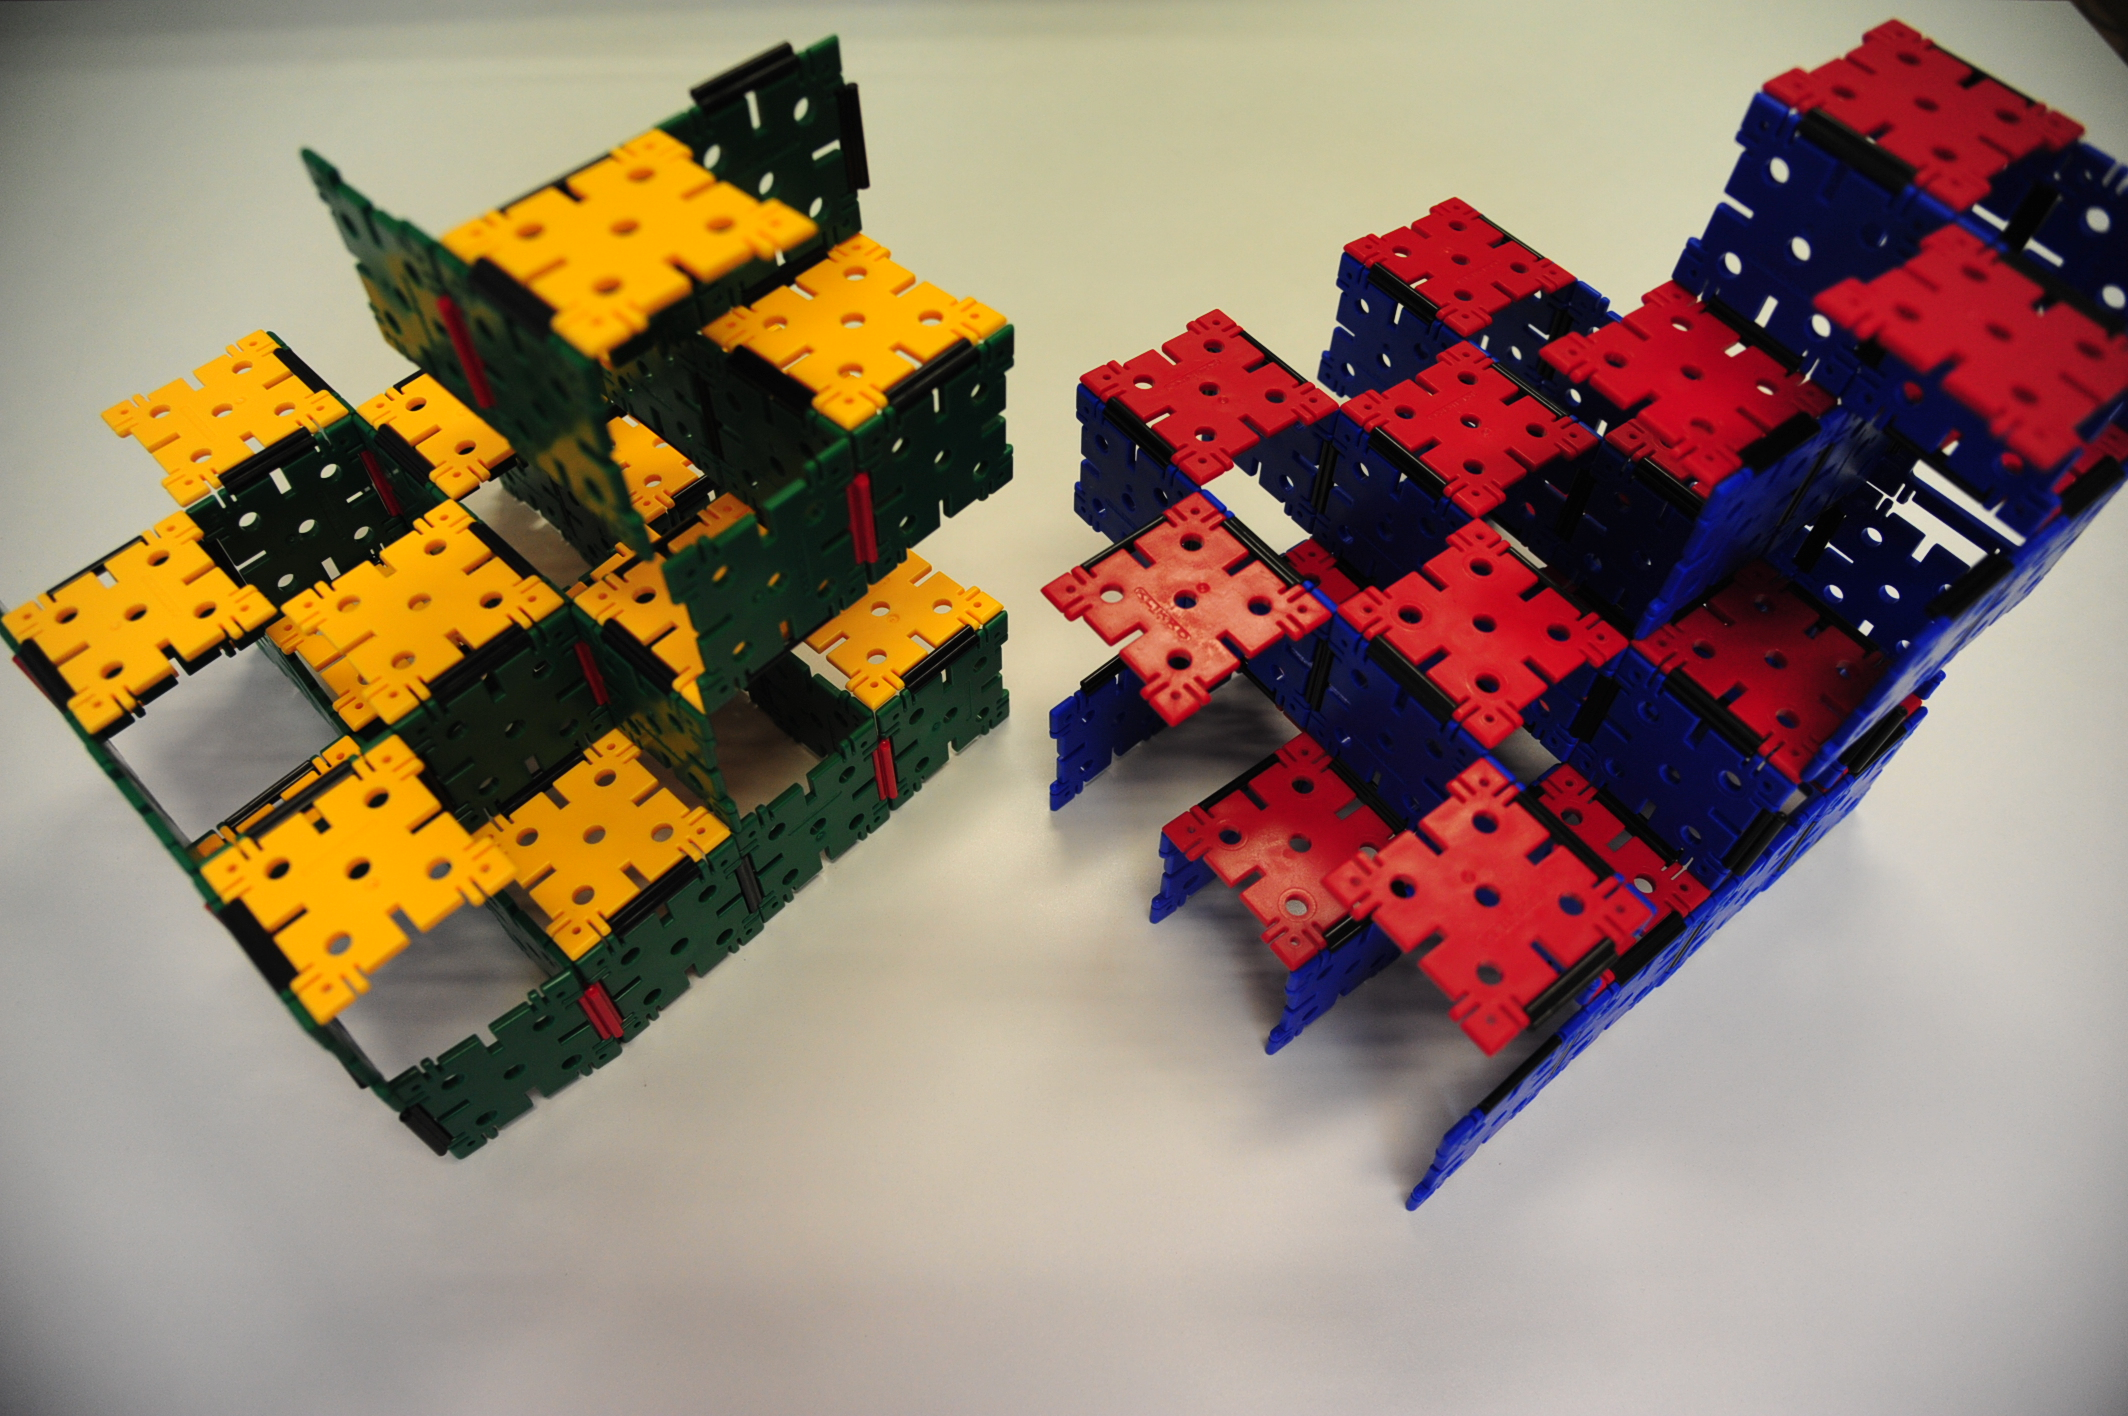
\includegraphics[height=4cm]{toys}
%		\end{center}
%	\end{column}
%	\begin{minipage}[t][0.5\textheight]{0.55\textwidth}
      \tableofcontents[currentsection]
%    \end{minipage}\hfill
%	\end{columns}
\end{frame}
}


% Delete this, if you do not want the table of contents to pop up at
% the beginning of each subsection:

\begin{document}

\begin{frame}
  \titlepage
\end{frame}

\begin{frame}{Collaborators}
  \begin{itemize}
  \item Tian Yuan: Fudan University.
  \item Chen Fang: Institute of Physics, CAS.
\end{itemize}
\vspace{4em}
\begin{center}
        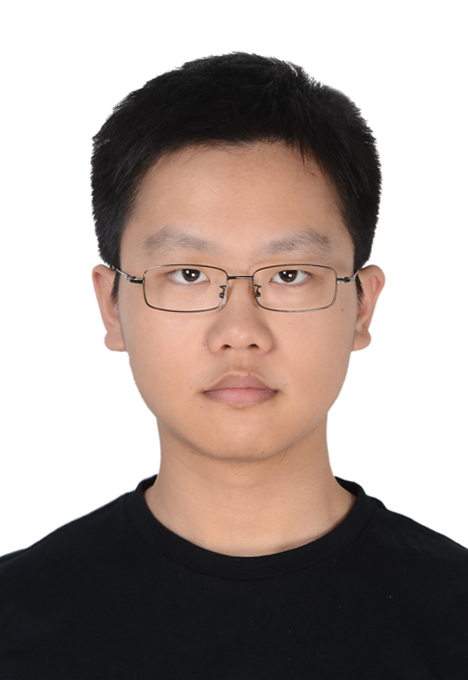
\includegraphics[height=3.5cm]{../people/tianyuan}~~~~
      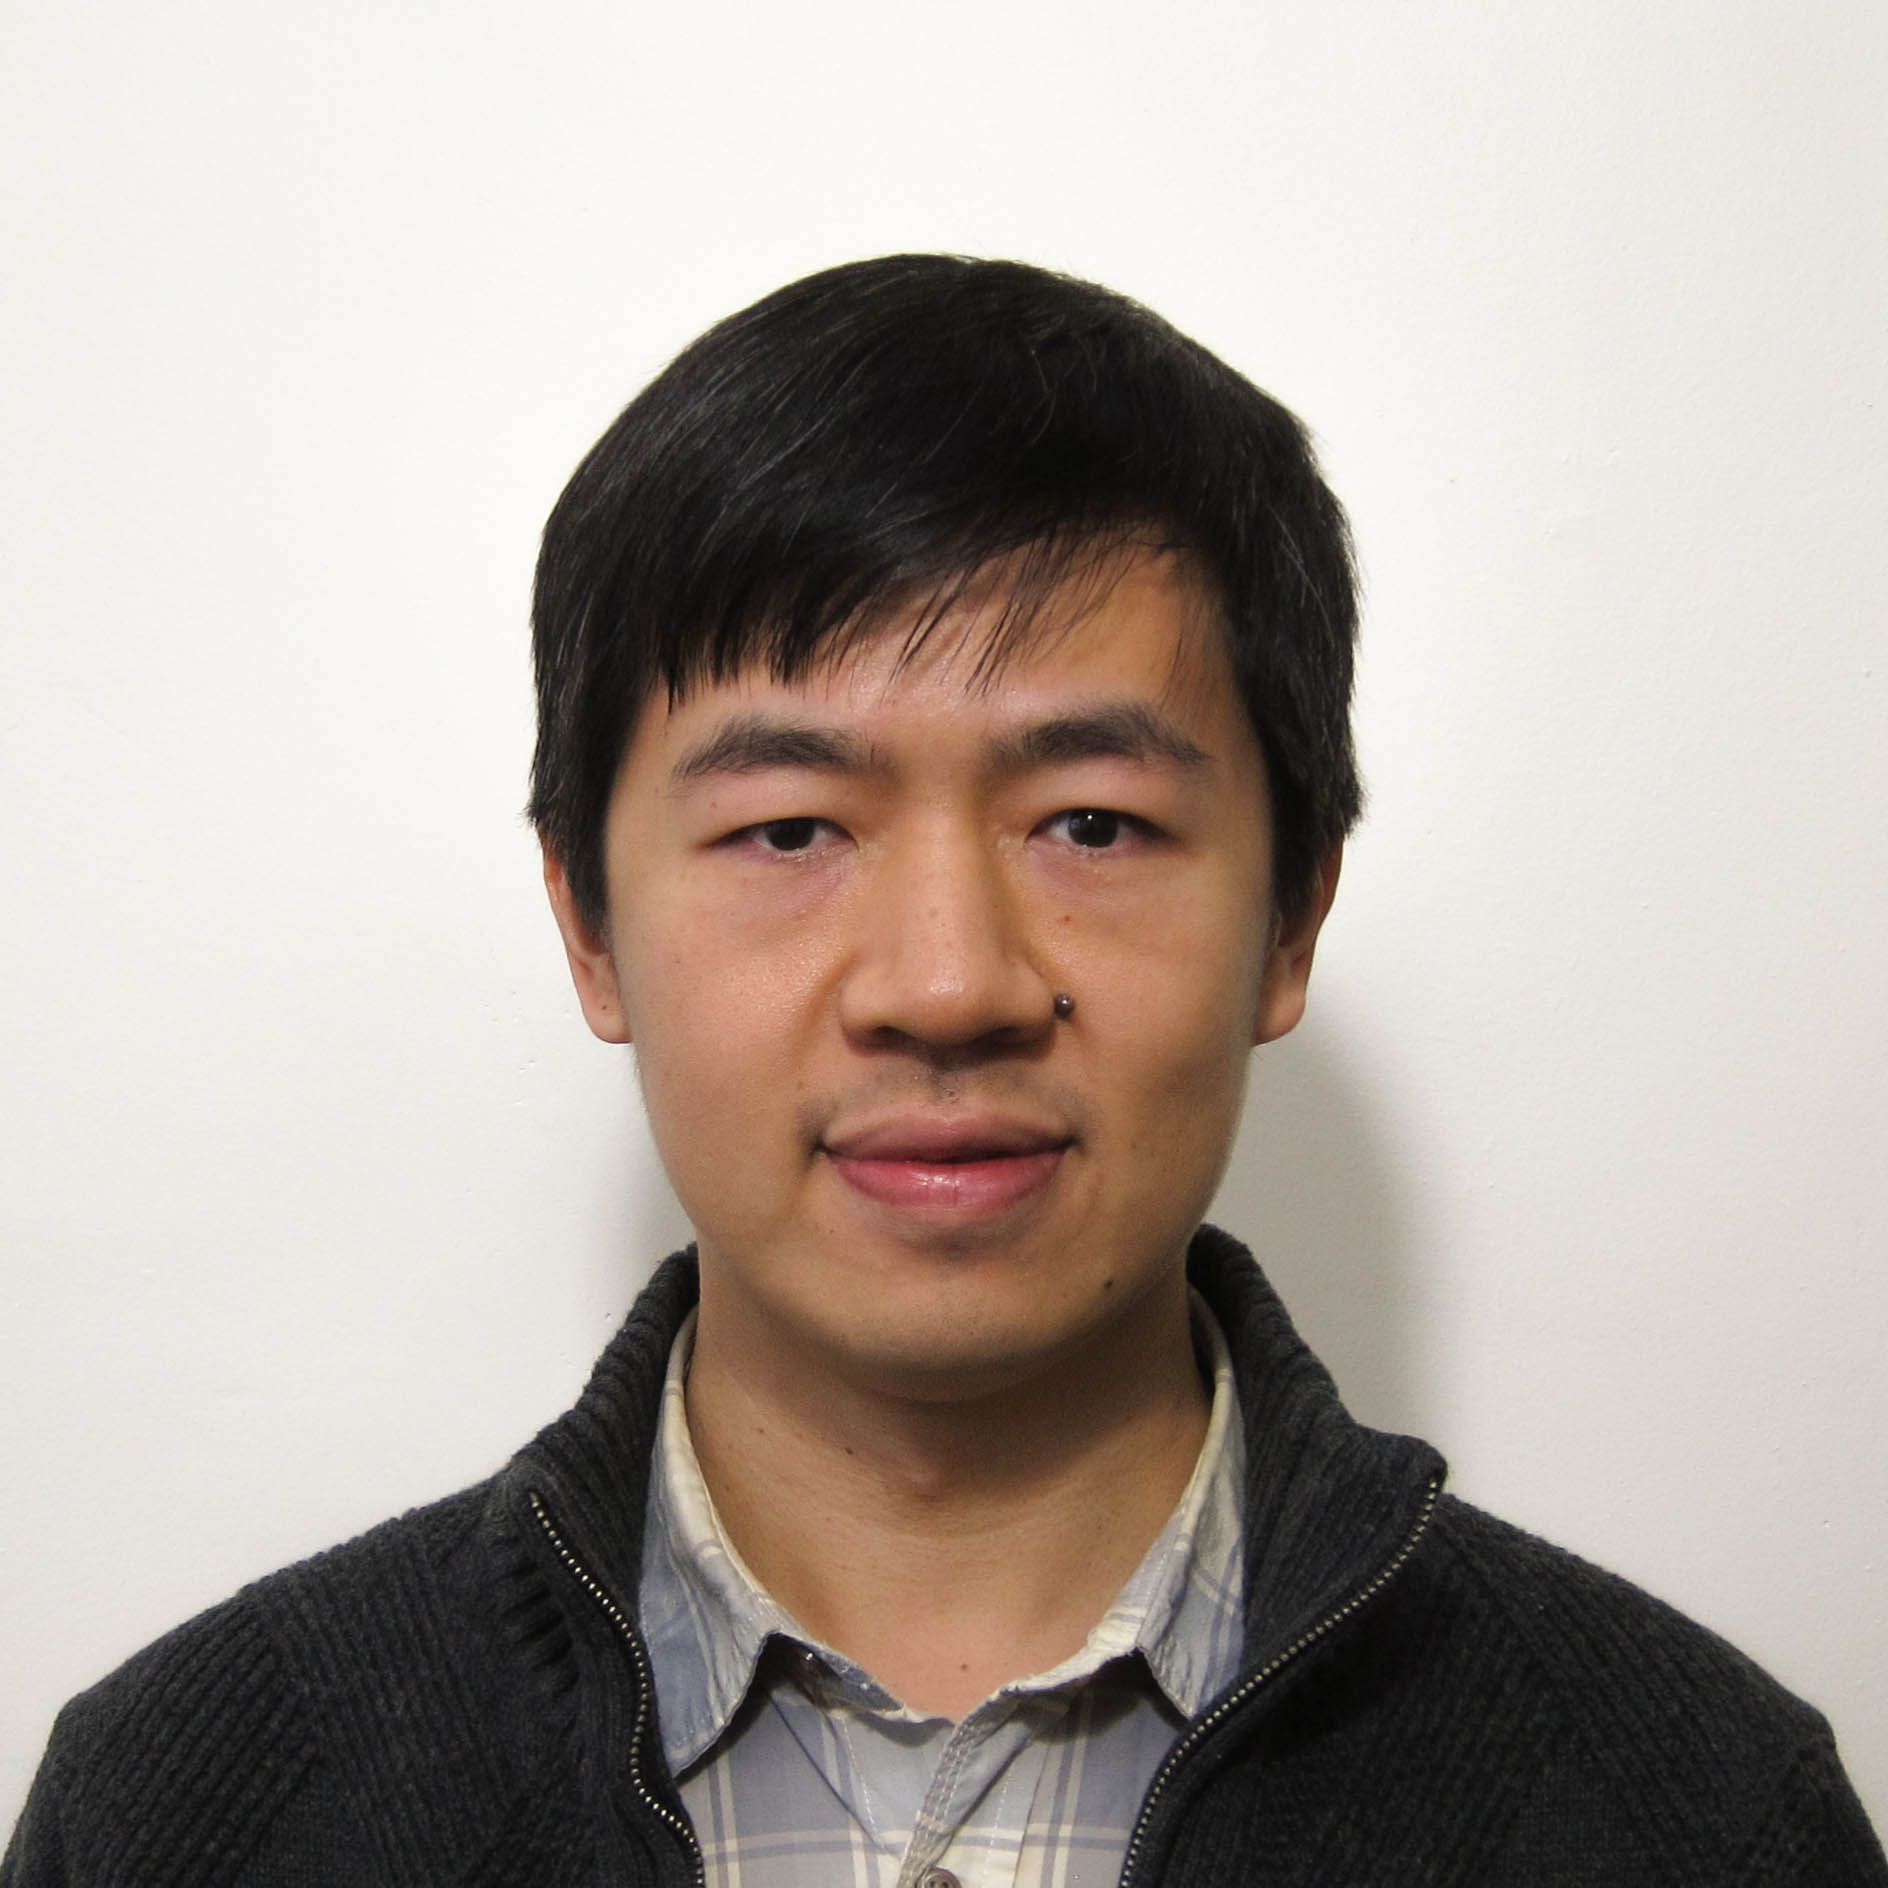
\includegraphics[height=3.5cm]{../people/chenfang}
    \end{center}
\end{frame}

\begin{frame}{Outline}
%	\begin{columns}
%		\begin{column}[t]{.45\textwidth}
%		\begin{center}
%			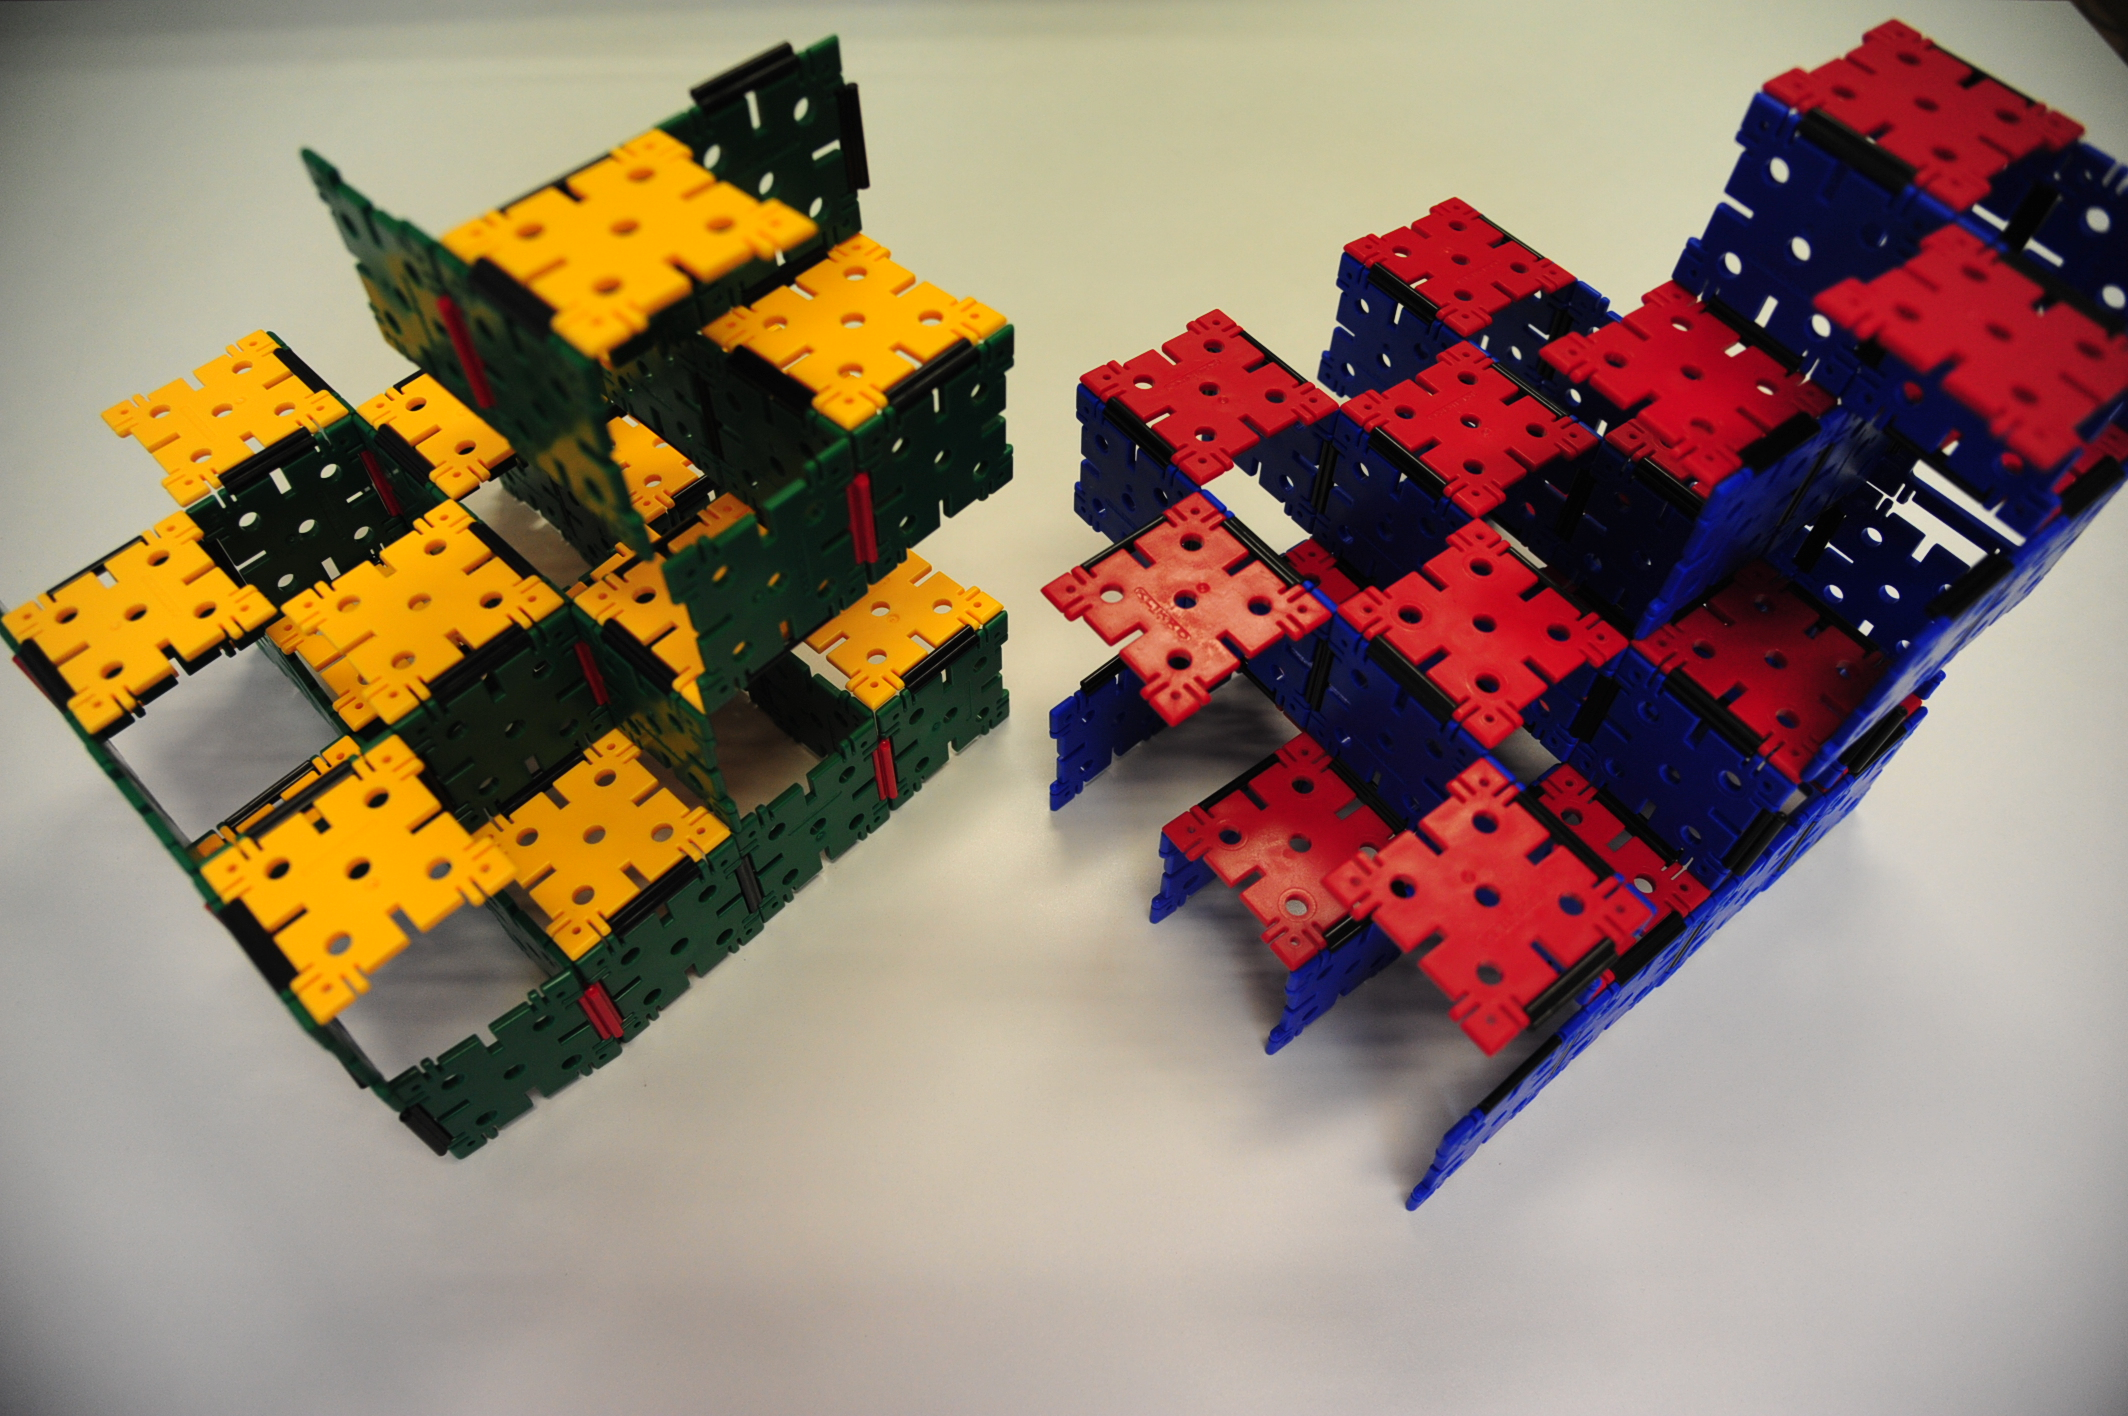
\includegraphics[height=4cm]{toys}
%		\end{center}
%	\end{column}
%	\begin{minipage}[t][0.5\textheight]{0.55\textwidth}
      \tableofcontents
%    \end{minipage}\hfill
%	\end{columns}
\end{frame}


\section{Introduction to Topological Crystalline States (TCSs)}

\begin{frame}
  \frametitle{Symmetry-Protected Topological (SPT) phases}
  \begin{itemize}
  \item Landau paragidm: phases are classified by symmetry breaking.
    \begin{center}
      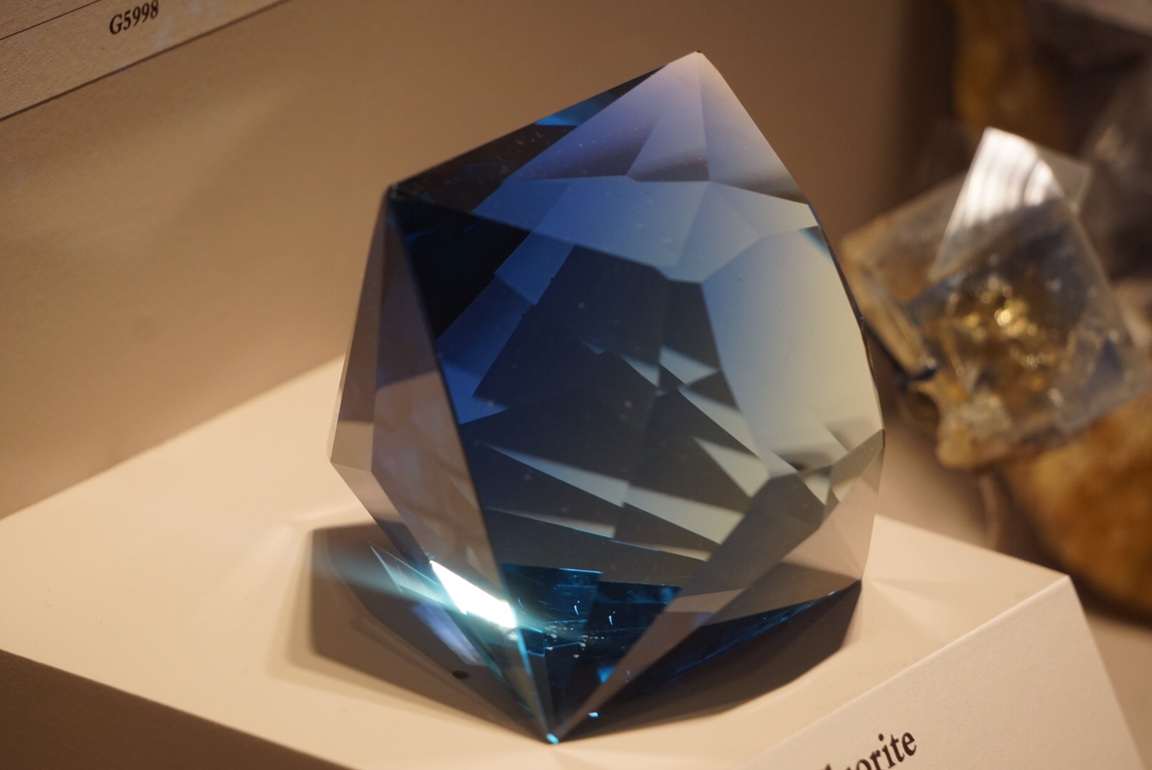
\includegraphics[height=1.5cm]{../resources/crystal}~~
      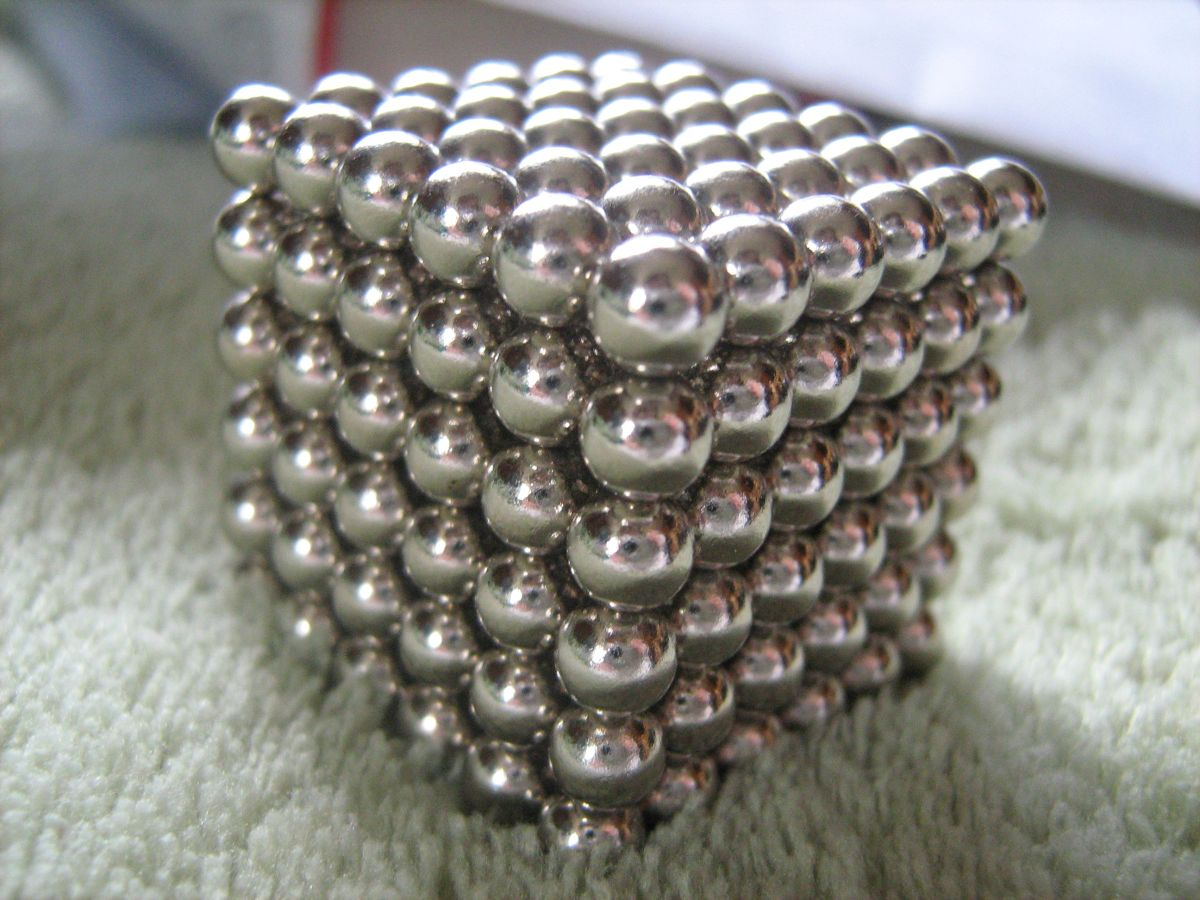
\includegraphics[height=1.5cm]{../resources/magnet}~~
      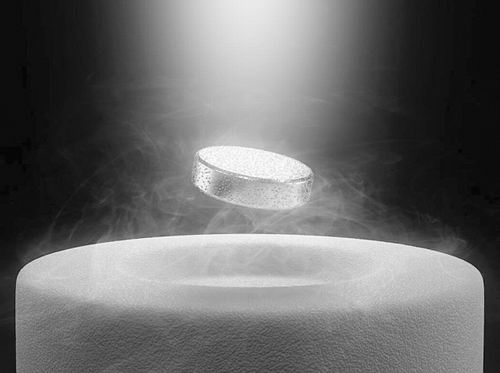
\includegraphics[height=1.5cm]{../resources/sc}
    \end{center}
  \item SPT: gapped topological phases beyond Landau paradiam.
  \item Gapped bulk : cannot be smoothly connected to a trivial state without closing gap or breaking symmetry.
  \item Symmetry-protected gapless surface states.
  \item Example: integer quantum Hall states; topological insulators.
    \begin{center}
      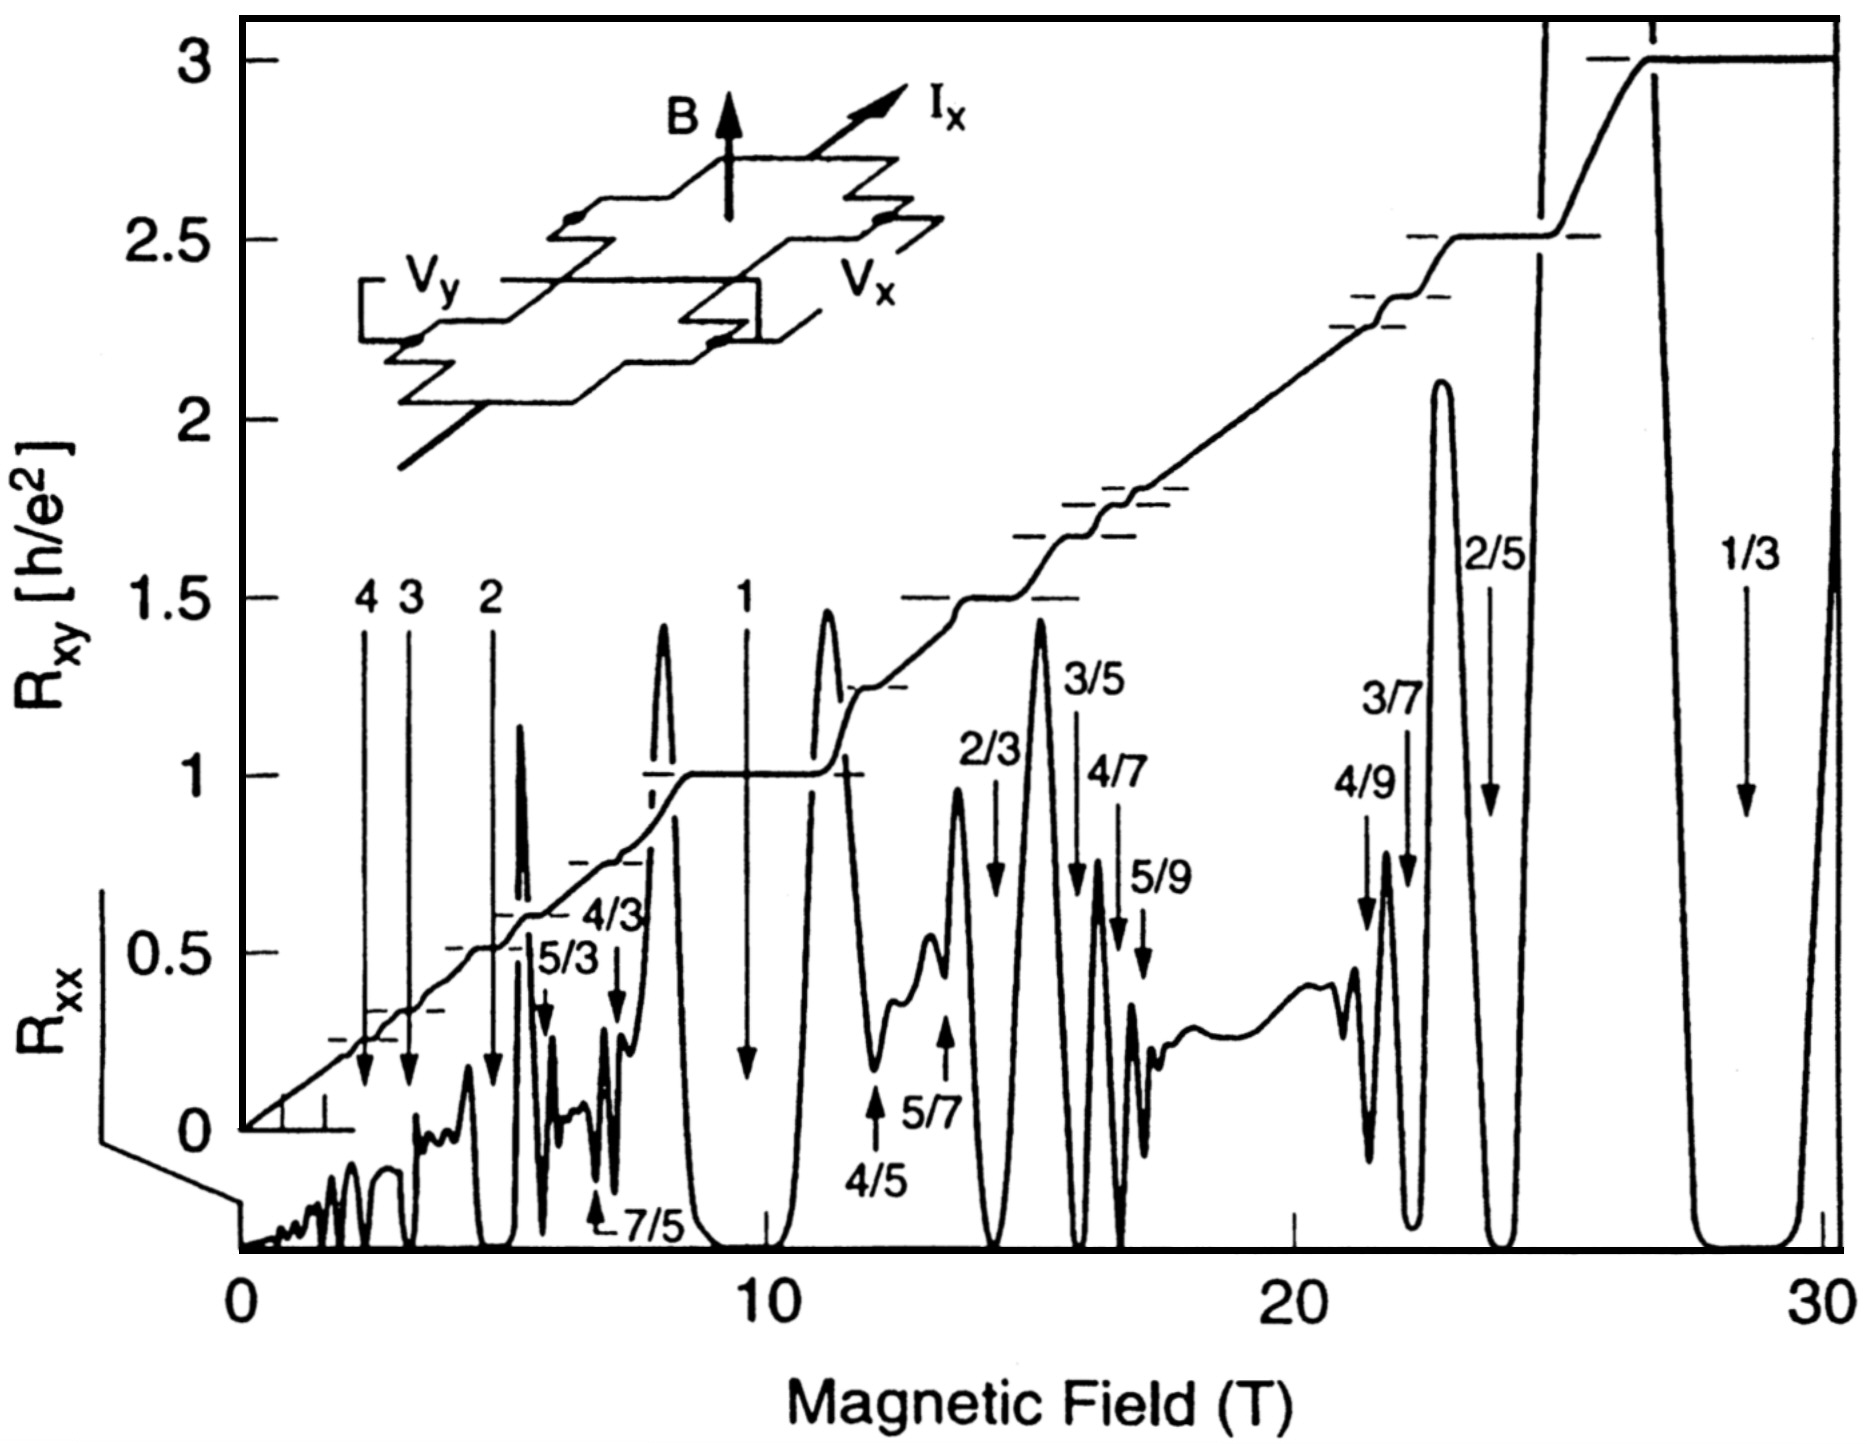
\includegraphics[height=2cm]{../resources/fqhe}~~
      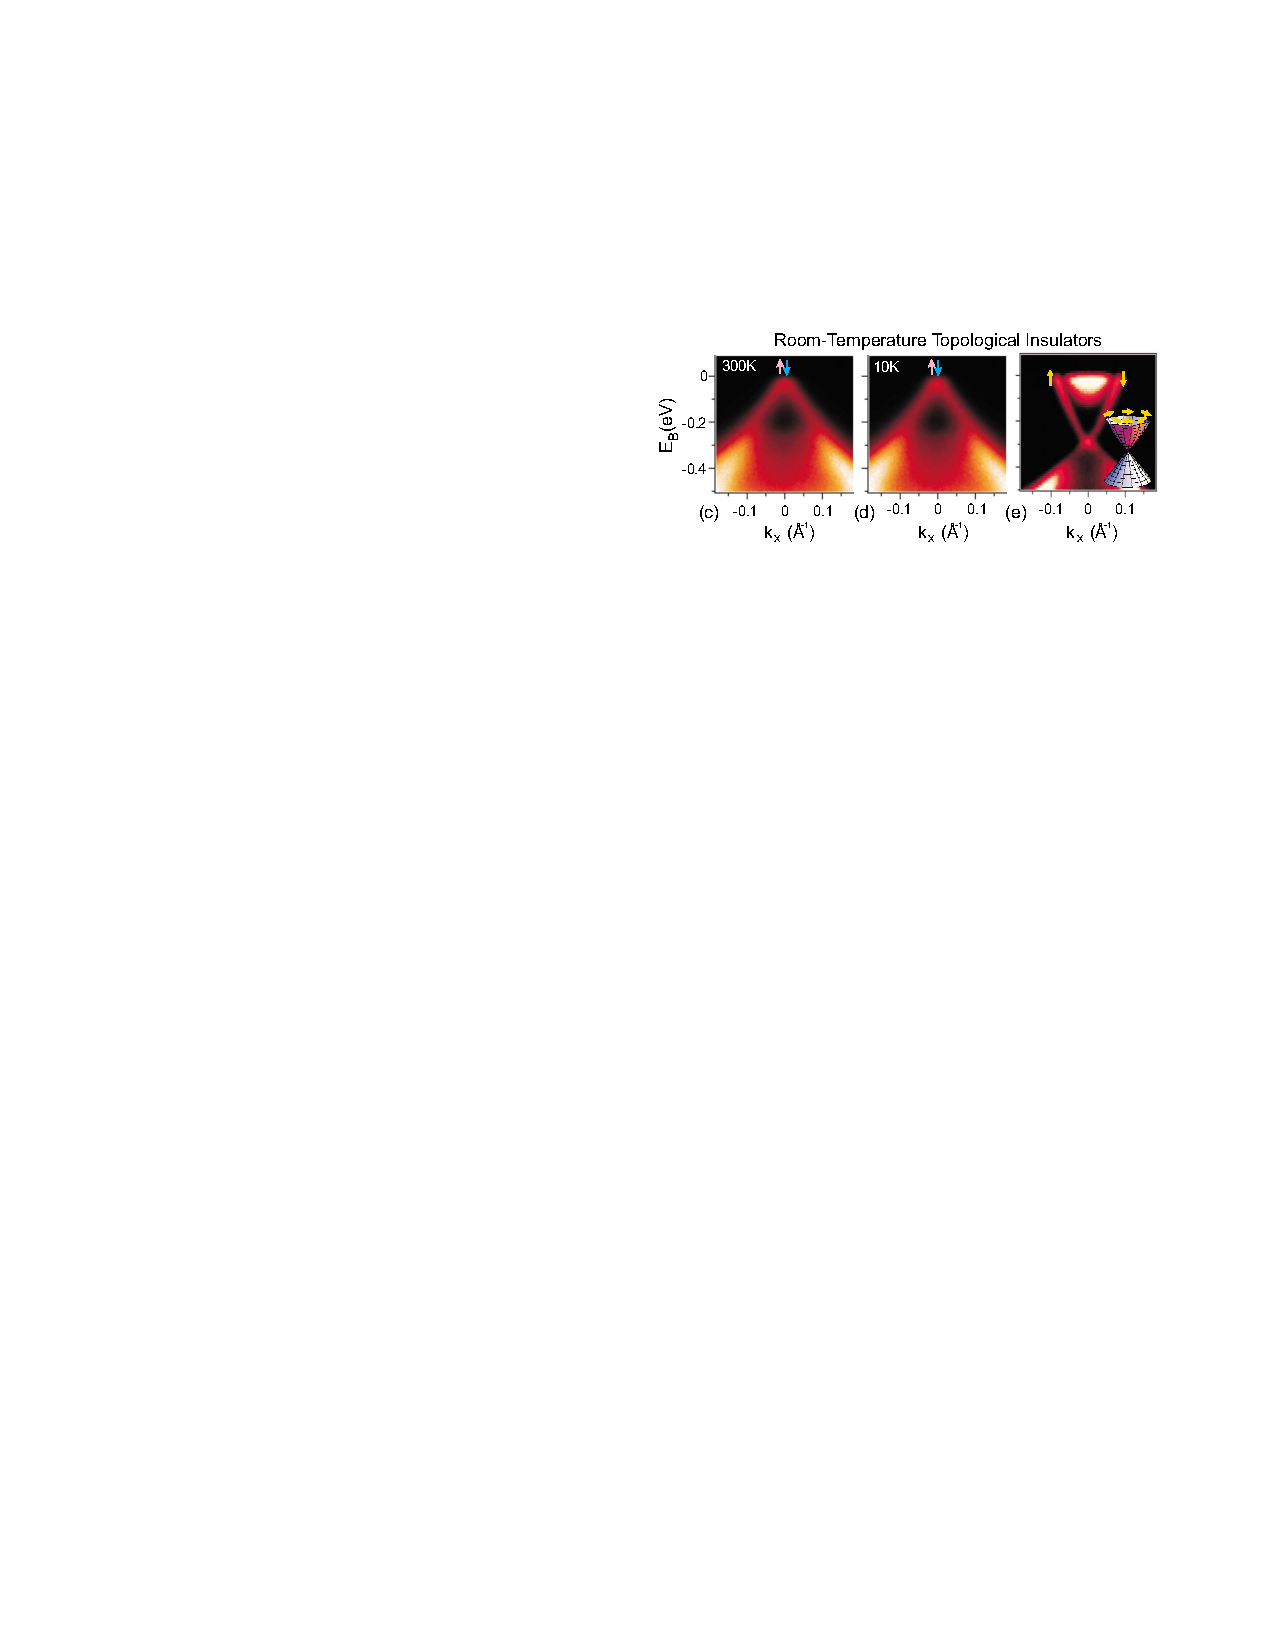
\includegraphics[height=2cm]{../spspt/ti_surface}
    \end{center}
  \end{itemize}
\end{frame}

\begin{frame}{Topological Crystaline States = Space-group SPT}
  \begin{itemize}
    \item<1-> Example: Topological Crystalline Insulators.
    \item<2-> High-order surface states.
    \emph{TCS = high-order topological states.}
    \begin{enumerate}
      \item<3-> $0^{th}$ order: 2d surface state. Strong SPT states.
      \item<4-> $1^{st}$ order: 1d hinge state.
      \item<5-> $2^{nd}$ order: 0d corner state.
      \item<6-> $3^{th}$ order: no surface state. Atomic insulator (AI).
    \end{enumerate}
  \end{itemize}
  \begin{center}
    \begin{tikzpicture} [scale=2]
      \fill<3-> [blue!50] (0,0)--(1,0)--(1.5,.5)--(1.5,1.5)--(0.5,1.5)--(0,1)--(0,0);
      \draw<4> [thick,red] (0,0)--(1,0)--(1,1)--(0,1)--(0,0);
      \draw<4> [thick,red] (1,0)--(1.5,.5)--(1.5,1.5)--(1,1);
      \draw<4> [thick,red] (1.5,1.5)--(0.5,1.5)--(0,1);
      \draw<4> [thick,red] (0,0)--(.5,.5)--(.5,1.5);
      \draw<4> [thick,red](.5,.5)--(1.5,.5);
      \draw<5-> [thick] (0,0)--(1,0)--(1,1)--(0,1)--(0,0);
      \draw<5-> [thick] (1,0)--(1.5,.5)--(1.5,1.5)--(1,1);
      \draw<5-> [thick] (1.5,1.5)--(0.5,1.5)--(0,1);
      \draw<5-> [thick] (0,0)--(.5,.5)--(.5,1.5);
      \draw<5-> [thick](.5,.5)--(1.5,.5);
      \fill<5-> [red] (0,0) circle (2pt);
      \fill<5-> [red] (1,0) circle (2pt);
      \fill<5-> [red] (0,1) circle (2pt);
      \fill<5-> [red] (1,1) circle (2pt);
      \fill<5-> [red] (0.5,0.5) circle (2pt);
      \fill<5-> [red] (1.5,0.5) circle (2pt);
      \fill<5-> [red] (0.5,1.5) circle (2pt);
      \fill<5-> [red] (1.5,1.5) circle (2pt);
    \end{tikzpicture}      
  \end{center}
\end{frame}

\begin{frame}{Why Topological Crystaline States?}
  \begin{itemize}
    \item Crystalline symmetries are present in all solid-state materials.
    \item High-order boundary states: TCSs (excluding the Atomic Insulators) are a.k.a. High-Order Topological States.
    May be useful for storing quantum information.
  \end{itemize}
  \begin{center}
    \begin{tikzpicture} [scale=2]
      \fill [blue!50] (0,0)--(1,0)--(1.5,.5)--(1.5,1.5)--(0.5,1.5)--(0,1)--(0,0);
      \draw [thick,red] (0,0)--(1,0)--(1,1)--(0,1)--(0,0);
      \draw [thick,red] (1,0)--(1.5,.5)--(1.5,1.5)--(1,1);
      \draw [thick,red] (1.5,1.5)--(0.5,1.5)--(0,1);
      \draw [thick,red] (0,0)--(.5,.5)--(.5,1.5);
      \draw [thick,red](.5,.5)--(1.5,.5);
      \fill [red] (0,0) circle (2pt);
      \fill [red] (1,0) circle (2pt);
      \fill [red] (0,1) circle (2pt);
      \fill [red] (1,1) circle (2pt);
      \fill [red] (0.5,0.5) circle (2pt);
      \fill [red] (1.5,0.5) circle (2pt);
      \fill [red] (0.5,1.5) circle (2pt);
      \fill [red] (1.5,1.5) circle (2pt);
    \end{tikzpicture}      
  \end{center}
\end{frame}

\begin{frame}
    \frametitle{Classification of Topological Crystaline States}
    \begin{itemize}
    \item Two approaches:
      \begin{enumerate}
      \item Thorngren and Else (2018): the crystalline equivalence principle
        \[SG\simeq G;\quad \mathcal H^D(SG)\simeq\mathcal H^D(G).\]
      \item Real-space recipes: Zhida Song, Chen Fang and YQ, Nat. Commun. (2020).\\
        \emph{Examples: mirror SPT, weak SPT (translation symmetry).}
        %\emph{Patch construction: Zhida Song, Shengjie Huang, YQ, Chen Fang and Michael Hermele, Sci. Adv. 5, eaax2007 (2019).}
      \end{enumerate}
    \item How to analyze high-order surface states?\\
      \emph{Case-by-case study of certain surface geometries?}
    \end{itemize}
    \begin{center}
    \begin{tikzpicture}[scale=.9]
    \fill [blue!20] (0,0)--(1,1)--(1,3)--(0,2)--(0,0);
    \draw (0,0)--(0,2)--(1,3);
    \draw (-1.5,0)--(1.5,0)--(1.5,2)--(-1.5,2)--(-1.5,0);
    \draw (1.5,0)--(2.5,1)--(2.5,3)--(1.5,2);
    \draw (2.5,3)--(-.5,3)--(-1.5,2);
    \end{tikzpicture}
    \hspace{2em}
    \begin{tikzpicture}[scale=.9]
    \fill [blue!40,opacity=.5] (0,0)--(1,1)--(1,3)--(0,2)--(0,0);
    \draw (0,0)--(0,2)--(1,3);
    \fill [blue!40,opacity=.5] (.5,0)--(1.5,1)--(1.5,3)--(0.5,2)--(0.5,0);
    \draw (.5,0)--(.5,2)--(1.5,3);
    \fill [blue!40,opacity=.5] (1,0)--(2,1)--(2,3)--(1,2)--(1,0);
    \draw (1,0)--(1,2)--(2,3);
    \fill [blue!40,opacity=.5] (-.5,0)--(.5,1)--(.5,3)--(-0.5,2)--(-0.5,0);
    \draw (-.5,0)--(-.5,2)--(.5,3);
    \fill [blue!40,opacity=.5] (-1,0)--(0,1)--(0,3)--(-1,2)--(-1,0);
    \draw (-1,0)--(-1,2)--(0,3);
    \draw (-1.5,0)--(1.5,0)--(1.5,2)--(-1.5,2)--(-1.5,0);
    \draw (1.5,0)--(2.5,1)--(2.5,3)--(1.5,2);
    \draw (2.5,3)--(-.5,3)--(-1.5,2);
    \end{tikzpicture}
    \end{center}
    \end{frame}
    
    \section{Anomaly pattern: where does the surface state appear}

    \begin{frame}{Anomaly Pattern of Point-Group Symmetry}
      \begin{itemize}
        \item<1-> Example: $G=C_4$.
        \item<2-> Gapped region: $X\subset S^2/G$; gapless region: $\bar X=(S^2/G) - X$.
        \item<2-> It is easier to study regions that can be gapped out.
        \item<3-> Deformation: G-equivariant map $X\rightarrow X'$.
        \begin{itemize}
          \item<4-> Minimal $X$: easy to study theoretically;
          \item<5-> Minimal $\bar X$: anomalous regions cannot be gapped out.
        \end{itemize}
        \item<6-> Results of $C_4$: three types of anomaly locations.
        \item<7-> Pure geometry: applies to free-fermion / bosonic / interacting-fermion SPTs.
      \end{itemize}
      \begin{center}
        \onslide<2->
        \begin{tikzpicture}[scale=1.2]
          \draw (0, 0) circle (1);
          %\draw (0, -1) to [out=30, in=-30] (0, 1) to [out=210, in=150] (0, -1);
          \filldraw [fill=black!30] (0, -1) to [out=30, in=-30] (0, 1) to [out=210, in=150] (0, -1);
          \fill [red] (0, 0.2) circle (0.3);
        \end{tikzpicture}
        \hspace{2em}
        \onslide<3->
        \begin{animateinline}{30}
          \multiframe{85}{Ra=0.05+0.01}{
            \begin{tikzpicture}[scale=1.2]
              \begin{scope}
              \path[draw, clip] (0, -1) to [out=30, in=-30] (0, 1) to [out=210, in=150] (0, -1);
              \fill[red] (-.6, -\Ra+0.1) to [out=-15, in=180+15] (.6, -\Ra+0.1) --
                (.6, \Ra+0.1) to [out=180+15, in=-15] (-.6, \Ra+0.1);
              \end{scope}
            \end{tikzpicture}
          }
        \end{animateinline}
        \hspace{4em}
        \onslide<6->
        \begin{tikzpicture}[scale=1.2]
          \fill [blue] (0, -1) circle (0.1);
          \fill [blue] (0, 1) circle (0.1);
          \path[draw, clip] (0, -1) to [out=30, in=-30] (0, 1) to [out=210, in=150] (0, -1);
          \draw[red, thick] (-.6, .05) to [out=-15, in=180+15] (.6, 0.05);
        \end{tikzpicture}
        \begin{tikzpicture}[scale=1.2]
          \draw (0, -1) to [out=30, in=-30] (0, 1) to [out=210, in=150] (0, -1);
          \draw [blue, thick] (0, -1) to [out=60, in=-60] (0, 1);
          \fill [red] (-0.2, 0) circle (0.1);
        \end{tikzpicture}
        \begin{tikzpicture}[scale=1.2]
          \fill [red] (0, 1) circle (0.1);
          %\fill [red] (0, -1) circle (0.1);
          \path[draw] (0, -1) to [out=30, in=-30] (0, 1) to [out=210, in=150] (0, -1);
        \end{tikzpicture}      
        \begin{tikzpicture}[scale=1.2]
          %\fill [red] (0, 1) circle (0.1);
          %\fill [red] (0, -1) circle (0.1);
          \path[draw, fill=blue] (0, -1) to [out=30, in=-30] (0, 1) to [out=210, in=150] (0, -1);
        \end{tikzpicture}
      \end{center}
    \end{frame}
  
    \begin{frame}{Computing the anomaly pattern}
      \begin{center}
        \begin{tikzpicture}[scale=1]
          %\fill [red] (0, 1) circle (0.1);
          %\fill [red] (0, -1) circle (0.1);
          \node at (-1.1, 0) {$X_1=$};
          \path[draw, fill=blue] (0, -1) to [out=30, in=-30] (0, 1) to [out=210, in=150] (0, -1);
        \end{tikzpicture}
        \hspace{2em}
        \begin{tikzpicture}[scale=1]
          \node at (-1.1, 0) {$X_2=$};
          \draw (0, -1) to [out=30, in=-30] (0, 1) to [out=210, in=150] (0, -1);
          \draw [blue, thick] (0, -1) to [out=60, in=-60] (0, 1);
          \fill [red] (-0.2, 0) circle (0.1);
        \end{tikzpicture}
        \hspace{2em}
        \begin{tikzpicture}[scale=1]
          \node at (-1.1, 0) {$X_3=$};
          \fill [blue] (0, -1) circle (0.1);
          \fill [blue] (0, 1) circle (0.1);
          \path[draw, clip] (0, -1) to [out=30, in=-30] (0, 1) to [out=210, in=150] (0, -1);
          \draw[red, thick] (-.6, .05) to [out=-15, in=180+15] (.6, 0.05);
        \end{tikzpicture}
        \hspace{2em}
        \begin{tikzpicture}[scale=1]
          \node at (-1.1, 0) {$X_4=$};
          \fill [red] (0, 1) circle (0.1);
          %\fill [red] (0, -1) circle (0.1);
          \path[draw] (0, -1) to [out=30, in=-30] (0, 1) to [out=210, in=150] (0, -1);
        \end{tikzpicture}      
      \end{center}
  
      \begin{itemize}
      \item Bulk classification: $K = \mathcal H^4(C_4\times G_0)$.
      \item $K_{X_i} := \{\text{States can be gapped out on } X_i\}$; $K=K_{X_1}\supset K_{X_2}\supset K_{X_3}\supset K_{X_4}$.
      \item $K_{X_1}/K_{X_2}$: strong TI; $K_{X_2}/K_{X_3}$: 1st-order; $K_{X_3}/K_{X_4}$: 2nd-order; $K_{X_4}$: atomic insulator.
      \item $K_{X_2}=\mathcal H^4(C_4\times G_0)/\mathcal H^4(G_0)$.
      \item $K_{X_4}=0$. (No AI)
      \item $K_{X_3}$: whether $M$ and $c_4Mc_4^{-1}$ can be smoothly connected.
      \item Examples of hinge states: C Fang and L Fu, Sci. Adv. 2019.
      \end{itemize}
    \end{frame}

    \begin{frame}{Checking if two states are smoothly connected}
      \begin{columns}
        \column{.7\textwidth}
        \begin{enumerate}
          \item<1-> $\forall A \in K_{X_2}$: $A$ can be gapped out at a generic point.
          \item<2-> Find a possible gapped boundary $M$ ($dM=A$) at a generic point.
          \item<3-> Compute $M'=c_4Mc_4^{-1}$.
          \item<4-> Check if $M$ and $M'$ are smoothly connected:
          \begin{itemize}
            \item If $M$ can be continuously deformed into $M'$.
            \item If $M$ and $M'$ can be separated by a gapped boundary.
            \item If $M-M'$ is a trivial 2d state.
          \end{itemize}
          If so, $A\in K_{X_3}$.
        \end{enumerate}
        \column{.3\textwidth}
        \begin{tikzpicture}[scale=2]
          \node<2-> at (-.6, .05)[left] {$M$};
          \node<3-> at (.6, .05)[right] {$M'$};
          \fill [blue] (0, -1) circle (0.1);
          \fill [blue] (0, 1) circle (0.1);
          \path[draw, clip] (0, -1) to [out=30, in=-30] (0, 1) to [out=210, in=150] (0, -1);
          \fill<2-> [red] (-.5, .03) circle (0.1);
          \fill<3-> [red] (.5, .03) circle (0.1);
          \draw<4->[red, thick] (-.6, .05) to [out=-15, in=180+15] (.6, 0.05);
        \end{tikzpicture}
      \end{columns}
    \end{frame}

    \begin{frame}{Two tasks in computing the anomaly pattern}
      \begin{enumerate}
        \item Reduction of symmetry:\\
        \emph{Check if a state can be gapped out when symmetry is reduced:}
        $$\mathcal H^D(G')\subset \mathcal H^D(G) \text{ for } G'\subset G$$
        \item Homotopy problem:\\
        \emph{Check if two gapped boundary states are connected:}
        $$M-gMg^{-1}\simeq 0 \in \mathcal H^{D-1}(G)$$
      \end{enumerate}
      Anomaly patterns can be computed using these two steps.
      \begin{center}
        \begin{tikzpicture}[scale=1]
          %\fill [red] (0, 1) circle (0.1);
          %\fill [red] (0, -1) circle (0.1);
          \node at (-1.1, 0) {$X_1=$};
          \path[draw, fill=blue] (0, -1) to [out=30, in=-30] (0, 1) to [out=210, in=150] (0, -1);
        \end{tikzpicture}
        \hspace{2em}
        \begin{tikzpicture}[scale=1]
          \node at (-1.1, 0) {$X_2=$};
          \draw (0, -1) to [out=30, in=-30] (0, 1) to [out=210, in=150] (0, -1);
          \draw [blue, thick] (0, -1) to [out=60, in=-60] (0, 1);
          \fill [red] (-0.2, 0) circle (0.1);
        \end{tikzpicture}
        \hspace{2em}
        \begin{tikzpicture}[scale=1]
          \node at (-1.1, 0) {$X_3=$};
          \fill [blue] (0, -1) circle (0.1);
          \fill [blue] (0, 1) circle (0.1);
          \path[draw, clip] (0, -1) to [out=30, in=-30] (0, 1) to [out=210, in=150] (0, -1);
          \draw[red, thick] (-.6, .05) to [out=-15, in=180+15] (.6, 0.05);
        \end{tikzpicture}
        \hspace{2em}
        \begin{tikzpicture}[scale=1]
          \node at (-1.1, 0) {$X_4=$};
          \fill [red] (0, 1) circle (0.1);
          %\fill [red] (0, -1) circle (0.1);
          \path[draw] (0, -1) to [out=30, in=-30] (0, 1) to [out=210, in=150] (0, -1);
        \end{tikzpicture}      
      \end{center}
    \end{frame}

    \section{Anomaly patterns for free-fermion SPTs}

    \begin{frame}{Free-fermion classification: Ten-fold way.}
      \begin{columns}
        \column{.4\textwidth}
        \begin{itemize}
        \item 10-fold way and Bott periodicity.
        \item TRS: $T^2=\pm1$;
        \item PHS: $C^2=\pm1$;
        \item Chiral symmetry: $S=TC$.
        \end{itemize}
        \column{.6\textwidth}{\small
          \begin{tabular}{c|ccc|cc|cccc}
            \hline
            Class & $T^2$ & $C^2$ & $S$ & Type & q & 0d & 1d & 2d & 3d\\
            \hline\hline
            A & 0 & 0 & 0 & $\mathbb C$ & 0 & $\mathbb Z$ & 0 & $\mathbb Z$ & 0\\
            AIII & 0&0&1 & $\mathbb C$&1 & 0 & $\mathbb Z$ & 0 & $\mathbb Z$\\
            \hline
            D & 0&+1&0 & $\mathbb R$&0 & $\mathbb Z_2$&$\mathbb Z_2$&$\mathbb Z$&0\\
            DIII & $-1$&+1&1 & $\mathbb R$&1 & 0&$\mathbb Z_2$&$\mathbb Z_2$&$\mathbb Z$\\
            AII & $-1$&0&0 & $\mathbb R$&2 & $\mathbb Z$&0&$\mathbb Z_2$&$\mathbb Z_2$\\
            CII & $-1$&$-1$&1 & $\mathbb R$&3 & 0&$\mathbb Z$&0&$\mathbb Z_2$\\
            C & 0&$-1$&0 & $\mathbb R$&4 & 0&0&$\mathbb Z$&0\\
            CI & +1&$-1$&1 & $\mathbb R$&5 & 0&0&0&$\mathbb Z$\\
            AI & +1&0&0 & $\mathbb R$&6 & $\mathbb Z$&0&0&0\\
            BDI & +1&+1&1 & $\mathbb R$&7 & $\mathbb Z_2$&$\mathbb Z$&0&0\\
            \hline
        \end{tabular}}
      \end{columns}
    \end{frame}

    \begin{frame}{Adding an onsite unitary symmetry}
      \begin{itemize}
        \item<1-> Why only TRS and PHS in 10-fold way?
        \item<2-> Free fermion + onsite unitary symmetry $G$: Hamiltonian is block-diagonalized into irreps of $G$:
        \[H=H_1\oplus H_2\oplus\cdots\begin{pmatrix}
          H_1 & 0 & 0\\
          0 & H_2 & 0\\
          0 & 0 & \cdots
        \end{pmatrix}\]
        \item<2-> Each block (each irrep) has a topological invariant.
        \item<3-> Real irreps: $\mathbb R$, $\mathbb C$ and $\mathbb H$-types.
        \item<3-> $\mathbb C$-type: $\mathrm{Cl}^{q+1,d}\rightarrow \mathbb{C}\mathrm{l}^{q+1+d}$;
        $\mathbb H$-type: $\mathrm{Cl}^{q+1,d}\rightarrow \mathrm{Cl}^{q+5,d}$.
        \item<4-> This solves the symmetry-reduction problem.
      \end{itemize}
    \end{frame}

    \begin{frame}{Homotopy problem: explicit form of Dirac mass terms}
      \begin{itemize}
        \item All free-fermion states can be constructed by Dirac Hamiltonians,
        \[H(k)=iM+\left(\sum_{n=1}^d k_n^2\right)iM_0+\sum_{n=1}^d k_n\tilde{\Gamma}_n\]
        \item $\tilde \Gamma_m^2$ and $M$ form a representation of a Clifford Algebra
        \[-M^2=\tilde \Gamma_m^2=I; \{M,\tilde\Gamma_m\}=0;
        \{\tilde\Gamma_m,\tilde\Gamma_n\}=2\delta_{mn}.\]
        \item $R=$ Space of $M$: represents different free-fermion states.
        \item $\pi_0(R)$ represents different phases.
        \item Use topological invariants to check if two different mass terms belong to the same element of $\pi_0(R)$:\\
        \emph{M Stone, C-K Chiu and A Roy, J. Phys. A: Math. Theor. 44 (2011) 045001.}
      \end{itemize}
    \end{frame}
      
    \begin{frame}{Example: class DIII}
      \begin{center}
        \begin{tikzpicture}[scale=1]
          %\fill [red] (0, 1) circle (0.1);
          %\fill [red] (0, -1) circle (0.1);
          \node at (-1.1, 0) {$X_1=$};
          \path[draw, fill=blue] (0, -1) to [out=30, in=-30] (0, 1) to [out=210, in=150] (0, -1);
        \end{tikzpicture}
        \hspace{2em}
        \begin{tikzpicture}[scale=1]
          \node at (-1.1, 0) {$X_2=$};
          \draw (0, -1) to [out=30, in=-30] (0, 1) to [out=210, in=150] (0, -1);
          \draw [blue, thick] (0, -1) to [out=60, in=-60] (0, 1);
          \fill [red] (-0.2, 0) circle (0.1);
        \end{tikzpicture}
        \hspace{2em}
        \begin{tikzpicture}[scale=1]
          \node at (-1.1, 0) {$X_3=$};
          \fill [blue] (0, -1) circle (0.1);
          \fill [blue] (0, 1) circle (0.1);
          \path[draw, clip] (0, -1) to [out=30, in=-30] (0, 1) to [out=210, in=150] (0, -1);
          \draw[red, thick] (-.6, .05) to [out=-15, in=180+15] (.6, 0.05);
        \end{tikzpicture}
        \hspace{2em}
        \begin{tikzpicture}[scale=1]
          \node at (-1.1, 0) {$X_4=$};
          \fill [red] (0, 1) circle (0.1);
          %\fill [red] (0, -1) circle (0.1);
          \path[draw] (0, -1) to [out=30, in=-30] (0, 1) to [out=210, in=150] (0, -1);
        \end{tikzpicture}      
      \end{center}
  
      \begin{itemize}
        \item Bulk classification: $\mathbb R[C_4]\simeq\mathbb R\oplus\mathbb R\oplus\mathbb C$;
        $A(\mathrm{Cl}^{2,3}\otimes\mathbb R[C_4])=\mathbb Z\oplus\mathbb Z\oplus\mathbb Z$.
        \item $K_{X_1}=\mathbb Z\oplus\mathbb Z\oplus\mathbb Z$.
        \item $K_{X_2}=A(\mathrm{Cl}^{q+1,3}\otimes\mathbb R[C_4])/A(\mathrm{Cl}^{q+1,3})=\mathbb Z\oplus\mathbb Z$.
        \item $K_{X_3}=2\mathbb Z\oplus\mathbb Z$.
        \item $K_{X_4}=0$.
        \item Strong TSC: $\mathbb Z$; 1st order: $\mathbb Z_2$; 2nd order: $2\mathbb Z\oplus\mathbb Z$; AI: 0.
      \end{itemize}
    \end{frame}

    \section{Anomaly patterns for interacting-fermion SPTs}

    \begin{frame}{Classification of interacting-fermion SPTs}
      \begin{itemize}
      \item Domain-wall decoration: Q.-R. Wang and Z.-C. Gu, PRX \textbf{10}, 031055 (2020).
      \item GAP package computing the classification: \url{www.github.com/yangqi137/SptSet}.
      \end{itemize}
      \begin{center}
      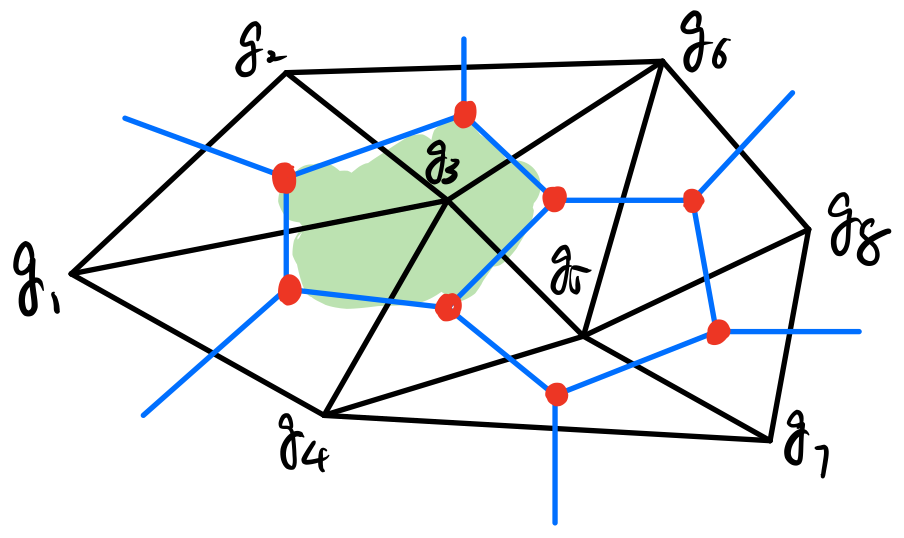
\includegraphics[width=.4\textwidth]{../chainmap/decoration.png}
      \end{center}
    \end{frame}
    
    \begin{frame}{Example: class DIII}
      \begin{center}
        \begin{tikzpicture}[scale=1]
          %\fill [red] (0, 1) circle (0.1);
          %\fill [red] (0, -1) circle (0.1);
          \node at (-1.1, 0) {$X_1=$};
          \path[draw, fill=blue] (0, -1) to [out=30, in=-30] (0, 1) to [out=210, in=150] (0, -1);
        \end{tikzpicture}
        \hspace{2em}
        \begin{tikzpicture}[scale=1]
          \node at (-1.1, 0) {$X_2=$};
          \draw (0, -1) to [out=30, in=-30] (0, 1) to [out=210, in=150] (0, -1);
          \draw [blue, thick] (0, -1) to [out=60, in=-60] (0, 1);
          \fill [red] (-0.2, 0) circle (0.1);
        \end{tikzpicture}
        \hspace{2em}
        \begin{tikzpicture}[scale=1]
          \node at (-1.1, 0) {$X_3=$};
          \fill [blue] (0, -1) circle (0.1);
          \fill [blue] (0, 1) circle (0.1);
          \path[draw, clip] (0, -1) to [out=30, in=-30] (0, 1) to [out=210, in=150] (0, -1);
          \draw[red, thick] (-.6, .05) to [out=-15, in=180+15] (.6, 0.05);
        \end{tikzpicture}
        \hspace{2em}
        \begin{tikzpicture}[scale=1]
          \node at (-1.1, 0) {$X_4=$};
          \fill [red] (0, 1) circle (0.1);
          %\fill [red] (0, -1) circle (0.1);
          \path[draw] (0, -1) to [out=30, in=-30] (0, 1) to [out=210, in=150] (0, -1);
        \end{tikzpicture}      
      \end{center}
  
      \begin{itemize}
        \item Bulk classification: $\mathcal H^4(\mathbb C_4\times\mathbb Z_2^T)=\mathbb Z_2\oplus\mathbb Z_4\oplus\mathbb Z_{16}$.
        \item $K_{X_1}=\mathbb Z_2\oplus\mathbb Z_4\oplus\mathbb Z_{16}$.
        \item $K_{X_2}=\mathcal H^4(\mathbb C_4\times\mathbb Z_2^T)/\mathcal H^4(\mathbb Z_2^T)=\mathbb Z_2\oplus\mathbb Z_4$.
        \item $K_{X_3}=\mathbb Z_4$: For each $\alpha\in K_{X_2}$, solve $d\beta=\alpha$ and check $\beta-c_4\beta c_4^{-1}\in \mathcal H^3(\mathbb Z_2^T)=\mathbb Z_2$.
        \item Strong TSC: $\mathbb Z_{16}$; 1st order: $\mathbb Z_2$; 2nd order: $\mathbb Z_4$; AI: 0.
        \item $K_{X_4}=0$.
      \end{itemize}
    \end{frame}
    \begin{frame}{Conclusion}
      \begin{itemize}
        \item Anomaly pattern: where gapless surface states may appear.
        \item Possible anomaly patterns can be enumerated for each point group: no need to study every surface geometry.
        \item Anomaly patterns can be computed for bosonic / fermionic SPT states.
      \end{itemize}
      \begin{center}
        \begin{tikzpicture}[scale=1]
          %\fill [red] (0, 1) circle (0.1);
          %\fill [red] (0, -1) circle (0.1);
          \node at (-1.1, 0) {$X_1=$};
          \path[draw, fill=blue] (0, -1) to [out=30, in=-30] (0, 1) to [out=210, in=150] (0, -1);
        \end{tikzpicture}
        \hspace{2em}
        \begin{tikzpicture}[scale=1]
          \node at (-1.1, 0) {$X_2=$};
          \draw (0, -1) to [out=30, in=-30] (0, 1) to [out=210, in=150] (0, -1);
          \draw [blue, thick] (0, -1) to [out=60, in=-60] (0, 1);
          \fill [red] (-0.2, 0) circle (0.1);
        \end{tikzpicture}
        \hspace{2em}
        \begin{tikzpicture}[scale=1]
          \node at (-1.1, 0) {$X_3=$};
          \fill [blue] (0, -1) circle (0.1);
          \fill [blue] (0, 1) circle (0.1);
          \path[draw, clip] (0, -1) to [out=30, in=-30] (0, 1) to [out=210, in=150] (0, -1);
          \draw[red, thick] (-.6, .05) to [out=-15, in=180+15] (.6, 0.05);
        \end{tikzpicture}
        \hspace{2em}
        \begin{tikzpicture}[scale=1]
          \node at (-1.1, 0) {$X_4=$};
          \fill [red] (0, 1) circle (0.1);
          %\fill [red] (0, -1) circle (0.1);
          \path[draw] (0, -1) to [out=30, in=-30] (0, 1) to [out=210, in=150] (0, -1);
        \end{tikzpicture}      
      \end{center}
    \end{frame}
\end{document}
